% Chapter 7

\chapter{Result} % Write in your own chapter title
\label{Chapter7}

\section{Experimental Set-up}
We used Mozilla and Eclipse bugs to measure the accuracy of our proposed
algorithm. We analysed the entire life span of both applications.  We divided our bug data sets into 10 folds and executed 9 iterations to cover all the folds.
Data collection. We used the bug reports to collect four kinds of data:
1. Keywords: we collect keywords from the bug description and
comments in the bug report.
2. Bug source: we retrieve the product and component the bug has been filed
under from the bug report.
3. Temporal information: we collect information about when the bug has
been reported and when it has been been fixed.
4. Developers assigned: we collect the list of developer IDs assigned to the bug

In our experiments, we varied the size of the test set, the
size of the vocabulary. The below graph shows the classification accuracy as a function of the train/test set split, when the full vocabulary
V of words found in bug reports is used.

\begin{figure}[hbt]
\begin{center}
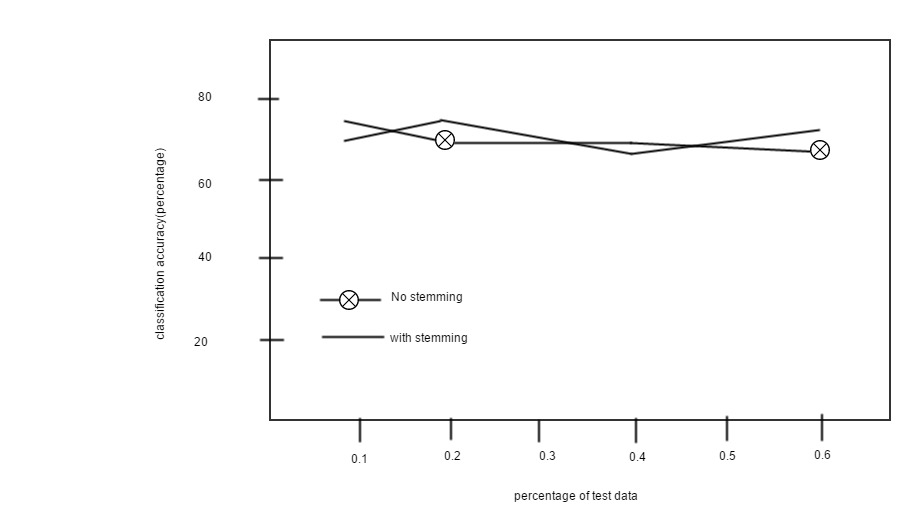
\includegraphics[height=15cm,width=15cm]{graph}
\caption{EXPERIMENTAL SET-UP}
\end{center}
\end{figure}


As we can see, the algorithm correctly assigns just under
75\% of the bugs, when 90\% of the document corpus is used
as training and 10\% as the test set. The accuracy slowly
declines to 65\% as the test set’s size is increased to 50% of
the corpus. 
\newline 

The graph also shows the results when the vocabulary was created using stemming, which identifies most grammatical variations of a word—such as “see”, “sees”, “seen”, for example—and treats them as a single term. The results are virtually unchanged, and any differences between the two conditions are within about one standard deviation at each data point.

Finally with 10 fold cross validation an accuracy of nearly 78\% is achieved and with linear SVM an accuracy of 80\% is achieved.